


\chapter{Electron Inertial Effects}
  \label{ch_inertia}

As laid out in \cref{ch_model}, Tuna resolves neither currents nor electric
fields parallel to the background magnetic field. This is unfortunate; parallel
electric fields generated by kinetic and inertial \Alfven waves (including
fundamental field line resonances\cite{rankin_1999,tikhonchuk_2000}) are a
topic of particular interest in the study of auroral particle precipitation. 

Parallel currents and electric fields can be added to Tuna through the
consideration of electron inertial effects in \ohmlaw:
\begin{align}
  0 &= \sz E_z - J_z &
  \text{becomes} & &
  \frac{1}{\nu} \ddt J_z &= \sz E_z - J_z
\end{align}

With the addition of the electron inertial term, it is necessary to track the
parallel current independent of the parallel electric field\footnote{The
parallel current $J_z$ is defined on the same points of the Yee grid as $E_z$.
It is offset in time by half of a time step. }. Solving by integrating
factors\footnote{The integrating factors technique is laid out explicitly for
\amplaw in \cref{sec_eqns}. } gives
\begin{align}
  J_3 &\assign J_3 \, \exp \arg{ - \nu \dt } +
    \dt \, \frac{n e^2}{\me} E_3 \, \exp \arg{ -\nu \tfrac{\dt}{2} }
\end{align}

From there, the parallel electric field can be updated directly;
\cref{e3_final} is replaced by the following: 
\begin{align}
  E_3 &\assign E_3 + c^2 \dt \, \lr{ g_{31} F^1 + g_{33} F^3 } -
    \frac{\dt}{\ez} J_3
\end{align}

The present section explores the complications that arise from the addition of
the electron inertial term to \ohmlaw, as well as a few results that may be
gleaned despite those complications. Notably --- for reasons discussed in
\cref{sec_lengths} --- the results presented in \cref{ch_results} do not make
use of the effects of electron inertia. 

Inertial effects have been considered in previous numerical work, such as by
Lysak and Song in 2001\cite{lysak_2001}, but never at the global scale. That
work considered waves in the ionospheric \Alfven resonator, with frequencies of
hundreds of \si{\mHz}, and did not account for the effects of the dipolar
geometry. In fact, in that work, circular polarization (essentially a
superposition of poloidal and toroidal modes) was noted to be a promising
avenue for future work. 

% -----------------------------------------------------------------------------
% -----------------------------------------------------------------------------
% -----------------------------------------------------------------------------
\section{The Boris Factor}
  \label{sec_boris}

With the addition of the electron inertial term, a cyclical dependence appears
between \amplaw and \ohmlaw:
\begin{align}
  \ddt E_z &\sim -\frac{1}{\ez} J_z &
  & \text{and} & 
  \ddt J_z &\sim \frac{n e^2}{\me} E_z &
  & \text{so} &
  \frac{ \partial^2 }{ \partial t^2 } E_z &\sim -\op^2 E_z
\end{align}

That is, electron inertial effects come hand in hand with the plasma
oscillation. 

\begin{figure}[!htb]
  \centering
  \includegraphics[width=\textwidth]{figures/op.pdf}
  \caption[Plasma Frequency Profile]{
    The plasma frequency reaches a peak value just under \SI{e6}{\Hz} near the
    equator. Outside the plasmasphere, its value is closer to \SI{e4}{\Hz},
    which is still not well-resolved by Tuna's usual time step.  
  }
  \label{fig_op}
\end{figure}

As mentioned in \cref{ch_math} and shown in \cref{fig_op}, plasma oscillation
is quite fast --- several orders of magnitude smaller than Tuna's time step as
determined in \cref{sec_coords} (\about\SI{10}{\us}). This poses a conundrum.
At Tuna's usual time step, the plasma oscillation becomes unstable within
seconds\footnote{For stability, $\op \dt < 1$ is necessary. }. On the other
hand, reducing the time step by three orders of magnitude to resolve the plasma
oscillation is computationally infeasible; a run slated for an hour would
require six weeks to complete. 

As it happens, this problem can be solved by artificially increasing the
parallel electric constant above its usual value of \ez. Doing so lowers both
the speed of light and the plasma frequency within the simulation. This
technique --- and others like it --- has been widespread in numerical modeling
since it was presented by Boris in 1970\cite{boris_1970}. The following
paraphrases an argument by Lysak and Song\cite{lysak_2001}, outlining its
validity specifically in the case of electron inertial effects. 

Supposing that the current and electric field are oscillating at frequency
$\omega$, the parallel components of \amplaw and \ohmlaw can be written
\begin{align}
  - i \omega \ez E_z &= \oomz \lr{ \, \curl{B} \, }_z - J_z & -
    \frac{i \omega}{\nu} J_z &= \sz E_z - J_z
\end{align}

Then, eliminating the current, the parallel electric field can be related to
the curl of the magnetic field by\footnote{From \cref{def_basics},
$c^2 \equiv \frac{1}{\mz \ez}$ and $\sz \equiv \frac{n e^2}{\me \nu}$ and
$\op^2 \equiv \frac{n e^2}{\me \ez}$. }
\begin{align}
  \label{boris_criterion}
  \lr{ 1 - \frac{\omega^2 - i \nu \omega}{\op^2} } E_z &= \frac{c^2}{\op^2}
    \lr{ \nu - i \omega } \lr{ \, \curl{B} \, }_z
\end{align}

In \cref{boris_criterion}, $\frac{c}{\op}$ is the electron inertial length.
While the speed of light and the plasma frequency each depend on \ez, their
ratio does not. This allows an estimation of how much the model should be
affected by an artificially-large electric constant (and thus an
artificially-small plasma frequency). So long as
$\frac{\omega^2 - i \nu \omega}{\op^2}$ remains small compared to unity, the
model should behave physically. 

For waves with periods of a minute or so, even perhaps-implausibly large Boris
factors are allowed; for example, increasing \ez by a factor of \num{e6} gives
$\left| \frac{\omega^2 + i \omega \nu}{ \op^2 } \right| \lesssim 0.01$. 

%In some places, this causes the speed of light to fall below the \Alfven speed; R{\"o}nnmark\cite{ronnmark_2000} terms this behavior ``anisotropic vacuum.''

%\todo{Generalized \ohmlaw, in case we decide we need it. Could talk through why all of the other terms are OK to neglect.  
%\begin{align}
%  \vec{E} + \vec{U} \! \times \! \vec{B} & = 
%  \eta \vec{J} + \tfrac{\me}{n e^2} \lrb{
%    \tfrac{\partial}{\partial t} \vec{J} + \nabla \cdot \lr{ 
%      \vec{J} \, \vec{U} + \vec{U} \,\vec{J} +
%      \tfrac{1}{n e} \vec{J} \, \vec{J} } } +
%  \tfrac{1}{n e} \vec{J} \! \times \! \vec{B} -
%  \tfrac{1}{n e} \div{ \vec{P_e} }
%\end{align}
%}

% -----------------------------------------------------------------------------
% -----------------------------------------------------------------------------
% -----------------------------------------------------------------------------
\section{Parallel Currents and Electric Fields}
  \label{sec_jz}

As discussed in \cref{sec_implications}, parallel electric fields in this
regime are expected to be at least six orders of magnitude smaller than the
perpendicular electric fields. Numerical results show general agreement: in
\cref{fig_electric_field_snapshots}, the parallel electric field appears
comparable to its perpendicular counterparts only after its been scaled up by a
factor of \num{e6}. 
\begin{figure}[!htb]
  \centering
  \includegraphics[width=\textwidth]{figures/electric_field_snapshots.pdf}
  \caption[Electric Field Snapshots]{
    Parallel electric fields are smaller than perpendicular electric fields by
    about six orders of magnitude. As a result, parallel electric fields do not
    contribute significantly to $\curl{E}$ in \farlaw. 
  }
  \label{fig_electric_field_snapshots}
\end{figure}

As such, the inclusion of electron inertial effects does not appreciably impact
the simulation's gross behavior. In \farlaw, \curl{E} is unaffected, to the
extent that side-by-side magnetic field snapshots with and without electron
inertial effects are not visibly distinguishable (not shown). In a sense, this
is reassuring. It ensures that the present section does not cast doubt on the
results presented in \cref{ch_results}, where electron inertial effects are
neglected. 

Even if there is no significant feedback through \farlaw, it's informative to
consider the structures that arise in parallel currents and electric fields
driven by perturbations in the ring current. For example, in
\cref{fig_electric_field_snapshots}, the parallel electric field perturbation
(with maxima near the ionosphere) exhibits the opposite harmonic structure to
the perpendicular electric field components (which peak near the equator). 

\cref{fig_slice_1000km} shows how parallel currents lines up with the Poynting
flux over time. Four runs are shown, one per row. The horizontal axis is time,
and the vertical axis is latitude. The real and imaginary components of the
parallel current are shown in the first and third columns respectively, while
the second and fourth columns show the poloidal and toroidal Poynting flux.
Values are taken at an altitude of \SI{1000}{\km}. 

\begin{figure}[!htb]
  \centering
  \includegraphics[width=\textwidth]{figures/slice_1000km.pdf}
  \caption[Current and Poynting Flux at \SI{1000}{\km}]{
    Parallel current and Poynting flux is shown for four runs, one per row,
    measured at an altitude of \SI{1000}{\km}. The parallel current is
    overwhelmingly imaginary, which implies a connection to the toroidal mode.
    Appropriately enough, the structure of the parallel current (particularly
    at low modenumber) seems to resemble the structure of the toroidal mode
    more than it does that of the poloidal mode. This is likely because the
    toroidal mode, with its sharp gradients across $L$-shells, dominates
    $\lr{ \curl{B} }_z$. 
  }
  \label{fig_slice_1000km}
\end{figure}

Poloidal and toroidal fields are overwhelmingly real and imaginary
respectively, because they are separated from one another by an azimuthal
derivative (which carries a factor of $i$). However, when a wave's polarization
is rotated by the Hall conductivity, there is no accompanying rotation in the
complex plane --- this gives rise to an imaginary component of the poloidal
wave and a real component of the toroidal wave. 

In \cref{fig_slice_1000km}, the ionospheric conductivity is small, so the
imaginary component of the parallel current dominates. This implies a
connection between the parallel current and the toroidal mode, and indeed, the
two do exhibit qualitatively similarities. At $\azm = 4$ in particular, the
poloidal and toroidal Poynting fluxes are similar in strength much of the time,
yet the form of the parallel current strongly resembles that of the toroidal
Poynting flux over the poloidal.

The toroidal mode's dominant effect on the parallel current at small \azm is
not surprising. As shown in \cref{fig_electric_field_snapshots}, toroidal waves
vary sharply in $L$\footnote{The sharp definition in $L$ of the toroidal mode
compared to the poloidal mode is also the topic of significant discussion in
\cref{ch_results}. }. When the poloidal and toroidal magnetic fields are
comparable in magnitude, $\dd{x} B_y$ typically exceeds $\dd{y} B_x$ (at least
for $\azm \lesssim 32$). 

Whereas the imaginary component of the parallel current corresponds to that
carried into the ionosphere by \Alfven waves, its real component comes from
electric fields rotated by the Hall conductivity. \cref{fig_slice_100km} shows
the same four runs as \cref{fig_slice_1000km}, but measured at \SI{100}{\km},
the Earthward boundary of the simulation. At that point, the real and imaginary
components are similar in magnitude. 

\begin{figure}[!htb]
  \centering
  \includegraphics[width=\textwidth]{figures/slice_100km.pdf}
  \caption[Current and Poynting Flux at \SI{100}{\km}]{
    The above slices are taken from the same runs shown in
    \cref{fig_slice_1000km}, but at an altitude of \SI{100}{\km} instead of
    \SI{1000}{\km}. The primary difference between the two altitudes is the
    strength of the ionospheric Hall conductivity, which directly couples the
    poloidal and toroidal modes. The Hall-rotated fields give rise to a real
    component of the parallel current, the structure of which follows the
    poloidal Poynting flux (as it rotates to the toroidal mode). 
  }
  \label{fig_slice_100km}
\end{figure}

In \cref{fig_slice_100km}, as in \cref{fig_slice_1000km}, the imaginary
component of the parallel current preferrentially follows the toroidal Poynting
flux. This is particularly apparent at $\azm = 16$, where the poloidal Poynting
flux is clearly stronger, yet the structure of the imaginary current resembles
that of the toroidal Poynting flux. The real parallel current, on the other
hand, appears to follow the poloidal Poynting flux. 

Put another way, low-\azm poloidal waves seem to primarily give rise to
field-aligned currents only after being rotated to the toroidal mode by the
Hall conductivity. At high modenumber, the two modes contribute comparably
to the formation of parallel currents. 

%It's not clear whether this disparity is to be expected. Theoretical work surrounding parallel currents from inertial \Alfven waves has typically been concerned specifically with the shear mode\cite{lysak_2003,tikhonchuk_2000}. The guided (high-\azm) poloidal mode does a good imitation of a shear \Alfven wave, but still maintains some ability to propagate across $L$-shells --- this fact is visible in \cref{fig_electric_field_snapshots}, and is discussed at length in \cref{ch_results}. 

%\todo{Is this expected? Tikhonchuk\cite{tikhonchuk_2000} looks specifically at the toroidal mode when considering shear \Alfven waves. Does the poloidal mode count as compressional even when it's guided? In his 2001 paper, Lysak\cite{lysak_2001} talks about how circularly-polarized waves might be interesting. That would be a superposition of the poloidal and toroidal modes, right? In that paper, he's looking at modes with frequencies of \SI{1}{\Hz} or so, in the context of the IAR. Lysak and Song's 2003 paper\cite{lysak_2003} looks at the toroidal mode, also in the IAR (?). }

%\todo{Notably, the Poynting flux waveforms are rectified --- they primarily carry energy Earthward. The current, on the other hand, alternates between upward and downward flow. This effect presumably arises because the current is a linear quantity while the Poynting flux is quadratic: the electric and magnetic fields that make it up oscillate in phase, so their product is positive even when they are negative. NOTE: THIS WOULD BE A GREAT THING TO MENTION IF WE WERE TALKING ABOUT PHASE! }

It's also possible to consider the effect of parallel currents and electric
fields on the ionosphere's energy budget, per Poynting's theorem:
\begin{align}
  \ddt u &= -\div{E} - \vec{J} \cdot \vec{E}
\end{align}

\begin{figure}[!htb]
  \centering
  \includegraphics[width=\textwidth]{figures/power_density.pdf}
  \caption[Power Density at the Ionosphere]{
    While field-aligned currents can be of significant size, they are not
    particularly good at depositing energy in the ionosphere. Energy deposited
    by the Poynting flux matches closely with Joule dissipation from the
    perpendicular currents, while $J_z E_z$ is smaller by several orders of
    magnitude. 
  }
  \label{fig_power_density}
\end{figure}

The magnitude of the parallel current tops out over \SI{1}{\uA/\m\squared},
just shy of the up-to-tens of \si{\uA/\m\squared} inferred from ground
observations and seen in situ\cite{carlson_1998,karlsson_1996,samson_1996}.
However, this current is not a significant contributor to ionospheric Joule
dissipation. As shown in \cref{fig_power_density}, the energy deposited in the
ionosphere by the Poynting flux matches closely with the energy lost to Joule
dissipation --- as it should, to conserve energy. But, according to the model,
Pedersen and Hall are dominant. The parallel component of
$\vec{J} \cdot \vec{E}$ is smaller by several orders of magnitude. 

%\todo{Parallel electric fields, supposedly, only appear at high altitude. \cite{marklund_1997,carlson_1998}. }

%\todo{Integrate up a parallel electric field to see the potential difference. Compare to the relation seen by \cite{olsson_1996}, $J_\parallel \sim \Psi_\parallel$ by a proportionality constant of \SIrange{e-8}{e-10}{\S/\meter\squared}. }

% -----------------------------------------------------------------------------
% -----------------------------------------------------------------------------
% -----------------------------------------------------------------------------
\section{Inertial Length Scales}
  \label{sec_lengths}

It's not quite fair to compare the parallel and perpendicular contributions to
\curl{E} as is done in \cref{sec_jz}. Perpendicular electric fields are on the
order of \SI{1}{\mV/\m}, with wavelengths on the order of \SI{e5}{\km}; they
cause magnetic fields to change at a rate of around \SI{0.1}{\nT/\s}. Parallel
electric fields, closer to \SI{e-6}{\mV/\m}, would need to vary over length
scales of \SI{0.1}{\km} to match with that. 

Such scales are believable. The characteristic length scale of the plasma
oscillation is the electron inertial length, $\frac{c}{\op}$, which is on the
order of \SI{1}{\km} in the auroral ionosphere and \SI{0.1}{\km} in the
low-altitude plasmasphere. However, Tuna's grid out bottoms out closer to
\SI{10}{\km}. That is, with the inclusion of electron inertial effects, the
grid is too coarse to resolve all of the waves expected to be present. The
model is prone to instability as a result --- for example, ``wigglies'' are
visible in the bottom-left subplot of \cref{fig_slice_100km}. 

\cref{fig_inertial_length} shows a run with perpendicular resolution smaller
than the electron inertial length, side by side with an analogous run on the
typical grid described in \cref{ch_model}. In order to carry out the
inertial-scale run, several concessions were made to computational cost. The
run simulates only a duration of \SI{100}{\s} (other figures in the present
chapter, and those in \cref{ch_results}, show \SI{300}{\s}), and the grid
covers only the auroral latitudes from $L=5$ to $L=7$. 

\begin{figure}[!htb]
  \centering
  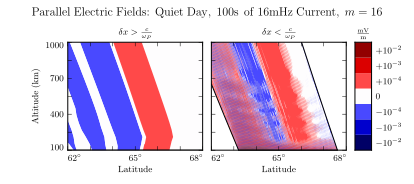
\includegraphics[width=\textwidth]{figures/inertial_length.pdf}
  \caption[Parallel Electric Fields by Perpendicular Grid Resolution]{
    The parallel electric field develops significant structure when the
    perpendicular grid resolution is smaller than the electron inertial
    length. Unfortunately, such runs are prohibitively expensive. The subplot
    on the right --- which still fails to resolve wave structure properly ---
    represents a 100-fold increase in computational time compared to that on
    the left. 
  }
  \label{fig_inertial_length}
\end{figure}

Even so, the run presents a significant computational expense. Spread over 16
cores, a \SI{100}{\s} run on Tuna's usual grid takes well under an hour. The
inertial-scale run barely finished in 96 hours, the cutoff at the Minnesota
Supercomputing Institute. This is because runtime goes as the inverse square of
grid resolution; not only does finer resolution require more grid cells, but it
also gives rise to proportionally smaller crossing times, imposing a smaller
time step. 

The snapshot shown in \cref{fig_inertial_length} uses a perpendicular grid
resolution of \SI{0.7}{\km} at the Earthward edge, which just satisfies the
Nyquist rate for the minimum inertial length of \SI{1.7}{\km}. It's still too
coarse. There is clearly some small-scale structure developing in the
ionosphere, but it's not well resolved. The large number of ``wigglies''
portends an imminent crash. 

% -----------------------------------------------------------------------------
% -----------------------------------------------------------------------------
% -----------------------------------------------------------------------------
\section{Discussion}

The present chapter is a proof of concept: the addition of electron inertial
effects to Tuna presents a promising first-principles-based approach to the
investigation of parallel currents and electric fields associated with field
line resonances. Electric fields arise which are consistent in magnitude with
those predicted by the dispersion relation, and parallel currents fall within
an order of magnitude or so of observed values, even when inertial length
scales are not properly resolved. 

Results in \cref{sec_jz} suggest a disparity between low-\azm poloidal and
toroidal FLRs in terms of the parallel current response. At low altitude, where
the two modes are directly coupled by the Hall conductivity, both seem to be
accompanied by parallel currents. However, in regions of low Hall conductivity,
parallel currents appear to preferrentially accompany toroidal waves. This is
likely a result of the toroidal mode's sharp gradients across $L$-shells. 

Future work  could consider the relationship between the dynamic
height-integrated potentials and the accompanying parallel currents,
specifically with respect to the Knight relation\cite{knight_1973}. Inertial
effects could also be accompanied by test particles, in order to gauge the
precipitation that would be expected to accompany global \Alfven{}ic potential
structures. 

Unfortunately, simulations are prone to instability when inertial length scales
are not properly resolved. And, at least at present, resolving those scales
poses a prohibitive computational expense. For this reason, the consideration
of inertial effects is limited to the present chapter; results in
\cref{ch_results} make use of the core version of Tuna presented in
\cref{ch_model}, which does not include the effects of electron inertia. 

Notably, the addition or omission of parallel currents and electric fields does
not appear to significantly alter the behavior of perpendicular electric fields
or magnetic fields. Because the parallel electric fields are relatively small,
$\curl{E}$ is essentially unaffected by their inclusion. Joule dissipation from
parallel currents also does not seem to be a significant in comparison to that
from Pedersen and Hall currents. 




